\section{Sprint 5: Autenticación}%Autenticación

\subsection{Descripción}

Este sprint tiene por objetivo definir un proceso de autenticación del usuario para con la API, sin importar el perfil del mismo, que garantice un nivel de seguridad adecuado para tranquilidad en el uso de la aplicación por parte de los interesados. 

\subsection{User Stories relacionados}

La \textbf{Tabla \ref{US-Sprint5}} indica las características de cada \textit{user story} relacionado, y servirá como guía fundamental para el desarrollo completo del sprint.

\begin{comment}
como usuario quiero contar con un acceso único y privado a mi información. Agregaría este user story, habría que ver la traza con el documento de diseño para que queden balanceados.
\end{comment}

\begin{table}[h]
	\centering
	\begin{tabular}{|m{1.5cm}|m{11.5cm}|}
		\hline
		\multicolumn{1}{|c|}{\textbf{ID}} &
		\multicolumn{1}{c|}{\textbf{Enunciado de la historia}} \\          
		\hline
		\textbf{US-\ref{modificarPermisos}} & Como \textbf{paciente}, quiero modificar los permisos de visualización de mis datos con respecto a cada uno de los integrantes del grupo familiar, para tener un control total sobre mi privacidad. \\
		\hline 
		\textbf{US-\ref{validarUsuario} } & Como \textbf{usuario}, quiero contar con un acceso único y privado a mi información. \\
		\hline 
	\end{tabular}
	\caption{Listado de \textit{User Stories} relacionados.}
	\label{US-Sprint5}
\end{table}


\subsection{Planificación}

\subsubsection{Período de realización}
\begin{itemize}
    \item \textbf{Inicio}: 11 de septiembre del 2015.
    \item \textbf{Fin}: 27 de septiembre del 2015.
\end{itemize}

\subsubsection{Sprint Backlog}

En la \textbf{Tabla \ref{Backlog-Sprint5}} se detalla el \textbf{Sprint Backlog} actual, indicando las tareas planificadas y efectuadas, en conjunto con el área a cargo de la misma, el responsable de la tarea, su descripción, \textit{user stories} relacionados, y tiempo de ejecución.

\begin{sidewaystable}
	\centering
		\begin{tabular}{|m{2.5cm}|>{\raggedright}m{2.5cm}|>{\raggedright}m{2.5cm}|m{7cm}|>{\centering\arraybackslash}m{1.5cm}|>{\centering\arraybackslash}m{1.5cm}|}
				\hline
				\textbf{Área a cargo} &
				\textbf{Responsable} &        
				\textbf{Revisor} &        	        
				\textbf{Tarea} &
				\textbf{US} &
				\textbf{Tiempo} \\
				\hline
				
				Backend& Michael Manganiello& Franco Canizo & Generación del modelo \texttt{User} y relación del mismo con el modelo \texttt{Profile}.  & US-\ref{modificarPermisos} \newline US-\ref{validarUsuario} & 13 horas
				\\ \hline
				Backend& Michael Manganiello& Franco Canizo & Generación del recurso relacionado con el modelo \texttt{User} y los métodos POST y GET que manejan los operadores HTTP correspondientes.  & US-\ref{modificarPermisos} \newline US-\ref{validarUsuario} & 11 horas
				\\ \hline
				Backend& Michael Manganiello & Franco Canizo& Generación del recurso para obtener un token para un usuario autenticado.  & US-\ref{modificarPermisos} \newline US-\ref{validarUsuario} & 9 horas
				\\ \hline
				Backend& Michael Manganiello & Franco Canizo& Creación del recurso \texttt{/my/profile}, que hace uso de la autenticación para obtener la información del perfil asociado al usuario. Permite los métodos GET y PUT. & US-\ref{modificarPermisos} \newline US-\ref{validarUsuario} & 4 horas
				\\ \hline
				Backend& Michael Manganiello & Franco Canizo& Creación de recursos GET: \texttt{/my/measurements} y \texttt{/my/measurements/latest}.
				
				Ambos recursos requieren autenticación (ya sea mediante usuario y contraseña, o token de sesión) y retornan las mediciones asociadas al perfil del usuario autenticado. Por lo tanto, no es necesario especificar un ID de perfil, sino que se toma el perfil del usuario que realiza la petición. & US-\ref{modificarPermisos} \newline US-\ref{validarUsuario} & 8 horas
				\\ \hline
				Frontend& Yanina Morales  & Iván Terreno& Cambio de las referencias a los recursos, para utilizar los que requieren que el usuario se encuentre logueado & US-\ref{modificarPermisos} \newline US-\ref{validarUsuario} & 12 horas
				\\ \hline
				Frontend& Yanina Morales  & Iván Terreno& Corrección de errores, para que el navbar sea responsive & US-\ref{modificarPermisos} \newline US-\ref{validarUsuario} & 8 horas
				\\ \hline		
		\end{tabular}
	\caption{\textit{Sprint Backlog}: Listado de tareas planificadas y efectuadas.}
	\label{Backlog-Sprint5}
\end{sidewaystable}



\subsection{Modelo de datos}

En la \textbf{Figura \ref{5-clase_autenticacion}} se detalla el diagrama de clases \textit{parcial}, utilizado durante el sprint actual.

\begin{figure}[h]
        \centering
        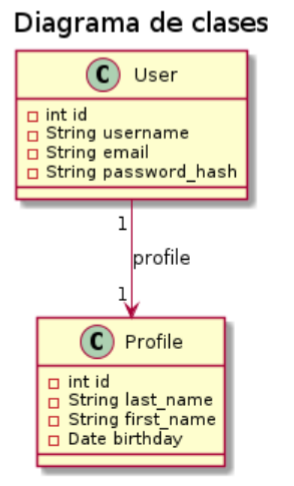
\includegraphics[width=0.3\textwidth]{img/clases_auth}
        \caption{Diagrama de clases, correspondiente a la autenticación.}
		\label{5-clase_autenticacion}
    \end{figure}


\subsection{Modelo funcional} 
La \textbf{Figura \ref{4-cu_autenticacion}} define el diagrama de casos de uso del presente sprint.

    \begin{figure}[h]
        \centering
        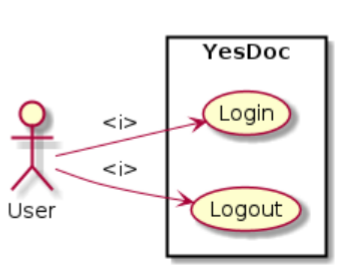
\includegraphics[width=0.4\textwidth]{img/cu_autenticacion}
        \caption{Diagrama de casos de uso, correspondiente a la autenticación.}
		\label{4-cu_autenticacion}
    \end{figure}


\subsubsection{Definición de modelos}

La definición del modelo \texttt{User} es bastante compleja, ya que define métodos para tomar la contraseña indicada y guardar exclusivamente su suma de verificación (\textit{hash}).
También se encarga de recibir contraseñas, y comparar con la suma de verificación existente, para autenticar la identidad de un usuario.

Por otro lado, define métodos para la generación y verificación del \textbf{token} asignado a un usuario.
Por último, define una relación uno a uno con el modelo \texttt{Profile}.


\subsubsection{Recursos}

El desafío en cuanto a la definición de recursos radica en que, según lo que establece \textbf{REST}, la restricción de que la API debe ser \textbf{\textit{stateless}} invalida la posibilidad de usar sesiones de usuario.

Esto es así para que permitir que la API sea escalable.
Es por ello que definimos una solución que se presenta en un punto gris entre puristas de REST y quienes realmente no hacen REST.

La solución consiste en generar un token para el usuario autenticado, el cual se almacena en las \textit{cookies} del cliente, y es usado en cada solicitud para autenticar al usuario.
Por esto, se definen recursos para dar de alta al usuario y para entregarle un token.

Las direcciones URL de los nuevos recursos de la API, se referencian en el \textbf{Listing \ref{recursos_api_autenticacion}}.

	\begin{lstlisting}[language=Python, caption=Listado de recursos añadidos por la API., label=recursos_api_autenticacion]
	api.add_resource(UserView, '/users/<int:id>')
	api.add_resource(UserList, '/users')
	api.add_resource(Token, '/token')
	api.add_resource(MyUserView, '/my/user')
	\end{lstlisting}

\subsection {Salidas del sistema}


\subsubsection{Solicitud POST al recurso de \texttt{Profile}}
    
	Para crear un usuario, debe existir un perfil creado.
	Para esto, usamos el recurso \texttt{/profiles} a través del método POST, y pasando como argumento los datos \texttt{first\_name}, \texttt{last\_name}, \texttt{birthday} y \texttt{gender\_id}.
	
\subsubsection{Solicitud POST al recurso de \texttt{User}}
    
    Realizamos ahora una solicitud HTTP, con método POST (utilizando \texttt{curl}) al recurso del usuario usando el ID del perfil creado previamente:

\begin{lstlisting}[language=bash]
curl -i http://localhost:5000/users -H "Content-Type: 
application/json" -X POST -d '{"username":"akathy", 
"email":"kathy@gmail.com", "password":"kathy1234", 
"profile_id":"2"}'
\end{lstlisting}
    
    Obtenemos la siguiente respuesta de la API, con un código 201.
    
\begin{lstlisting}[language=json]
HTTP/1.0 201 CREATED
Content-Type: application/json
Content-Length: 425
Server: Werkzeug/0.10.4 Python/2.7.6
Date: Tue, 20 Oct 2015 05:21:37 GMT

{
    "resource": {
        "email": "kathy@gmail.com", 
        "id": 2, 
        "profile": {
            "birthday": "1989-06-17", 
            "first_name": "Katherina", 
            "gender": {
                "description": "female gender", 
                "id": 2, 
                "name": "female"
            }, 
            "id": 2, 
            "last_name": "Aguirre"
        }, 
        "username": "akathy"
    }
}
\end{lstlisting}

\subsubsection{Solicitud POST al recurso \texttt{token}, mediante \textit{usuario} y \textit{contraseña}}
    
    Luego, con este usuario y contraseña, solicitamos un token al recurso correspondiente:

\begin{lstlisting}[language=bash]
curl -u akathy:kathy1234 http://localhost:5000/token
\end{lstlisting}
   
   Obtenemos así el token que debe ser almacenado en las \textbf{cookies}, tendrá una duración de 10 minutos y será utilizado en cada solicitud para autenticación.
   
\begin{lstlisting}[language=json]
{
    "resource": {
        "duration": 600, 
        "token": "eyJhbGciOiJIUzI1NiIsImV4cCI6MTQ0NTMxOTM3MCwiaWF0IjoxNDQ1MzE4NzcwfQ.eyJpZCI6Mn0.2eZRjbMq9tg4GykJx8EU-Ux4ZoyUW6WnBlADsvnpQvE"
    }
}
\end{lstlisting}


\subsection{Planificación de pruebas}

\subsubsection{Criterios de aceptación}

\begin{center}
\begin{longtable}{|m{0.5cm}|m{4cm}|m{4cm}|m{4.5cm}|}
\hline \rowcolor[gray]{0.9}
	\multicolumn{4}{|c|}{\textbf{Criterios de aceptación}} \\
    \hline  \rowcolor[gray]{0.9}
        \multicolumn{1}{|c|}{\textbf{ID}} &
        \multicolumn{1}{c|}{\textbf{Contexto}} &
        \multicolumn{1}{c|}{\textbf{Evento}} &
        \multicolumn{1}{c|}{\textbf{Resultado}} \\
    \hline
    \endhead
1&En caso de que exista un usuario registrado con el mismo nombre de usuario. & Al ejecutar el método POST del recurso \texttt{/users}.  & El sistema devolverá un JSON vacío y un código de error 400. \\ \hline
	\hline
2&En caso de que exista al menos un usuario registrado. & Al ejecutar el método GET del recurso \texttt{/users}  & El sistema devolverá una lista de JSON con los datos de los usuarios registrados. \\ 		\hline
	\hline
3&En caso de que exista un usuario registrado con el mismo correo electrónico. & Al ejecutar el método POST del recurso \texttt{/users}  & El sistema devolverá un JSON vacío y un código de error 400. \\ \hline
    \hline
4&En caso de que no exista un usuario registrado con el ID indicado & Al ejecutar el método GET/PUT del recurso \texttt{/users/id}  & El sistema devolverá un JSON con un mensaje de error y un código de error 404. \\ \hline

  \end{longtable}
\end{center}

\begin{comment}
	Cuando devolvería 401 el recurso del token.
\end{comment}



\subsubsection{Pruebas de seguridad }
\begin{center}
	\begin{longtable}{|m{4cm}|m{4cm}|m{3cm}|m{2cm}|}
		\hline \hline \rowcolor[gray]{0.9}
		\multicolumn{4}{|c|}{\textbf{Procedimiento de pruebas}} \\
		\hline 
		
		\multicolumn{4}{|c|}{\textbf{Descripción de escenario}: Debe hacer las pruebas un usuario no autenticado.} \\
		\hline 
		
		\rowcolor[gray]{0.9}
		\multicolumn{1}{|c|}{\textbf{Actor}} &
		\multicolumn{1}{c|}{\textbf{Sistema}} &
		\textbf{Resultado esperado}&
		\textbf{Resultado obtenido} \\
		\hline
		El usuario ingresa a la URL \url{https:// yesdoc.herokuapp.com/#/profileMeasurements}.
		&
		El sistema consulta a la API si el token se encuentra activo, la API devuelve un error 401 \textbf{[Figura \ref{no_autorizado_profile_measurement}]}.
		&
		Se redirige al usuario al formulario de login.
		&
		Correcto.
		\\ 
		\hline
		El usuario ingresa a la URL \url{https:// yesdoc.herokuapp.com/#/profileInformation}.
		&
		El sistema consulta a la API si el token se encuentra activo, la API devuelve un error 401 \textbf{[Figura \ref{no_autorizado_profile_measurement}]}.
		&
		Se redirige al usuario al formulario de login.
		&
		Correcto.
		\\ 
		\hline
		El usuario ingresa a la URL \url{https:// yesdoc.herokuapp.com/#/home}.
		&
		El sistema consulta a la API si el token se encuentra activo, la API devuelve un error 401 \textbf{[Figura \ref{no_autorizado_profile_measurement}]}.
		&
		Se redirige al usuario al formulario de login.
		&
		Correcto.
		\\ 
		\hline
				
	\end{longtable}
\end{center}

 \begin{figure}[h]
 	\centering
 	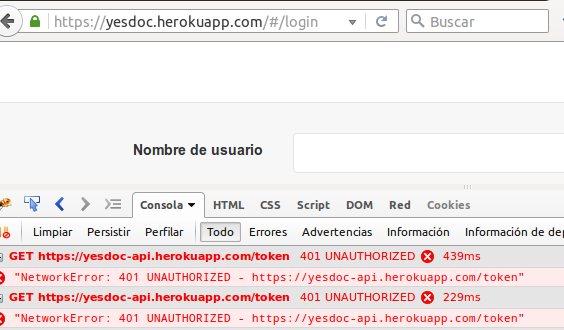
\includegraphics[width=0.6\textwidth]{img/no_autorizado_profile_measurement}
 	\caption{Acceso no autorizado a perfil de mediciones}
 	\label{no_autorizado_profile_measurement}
 \end{figure}
 
\subsection{Retroalimentación de pruebas}
En esta sección, se realizará una conclusión general de lo que se descubrió en las pruebas.

	\begin{itemize}
		\item \textbf{¿Qué fue bien?}
        	\begin{itemize}
				\item Las cargas y mediciones se llevan a cabo correctamente.
				\item Se restringe el acceso a usuarios no autenticados.
			\end{itemize}
   		\item \textbf{¿Qué se puede mejorar?}
        	\begin{itemize}
		        \item \textbf{Abierto}: Se podría avisar al visitante que debe autenticarse para poder ingresar.
            \end{itemize}
        

	\end{itemize}